\documentclass[12pt]{article}

%IMPORTS
\usepackage[catalan]{babel}
\usepackage[utf8]{inputenc}
\usepackage{graphicx}
\usepackage{wrapfig}
\usepackage{amsmath}
\usepackage{amssymb}
\usepackage{ragged2e} 
\usepackage{subfig}
\usepackage{caption}
\usepackage{subcaption}
\usepackage[usenames]{color}
\usepackage{xcolor}
\usepackage{float}
\usepackage{chngcntr}
\usepackage{ragged2e}
\usepackage{multirow}
\usepackage{vmargin}
\usepackage{hyperref}
\usepackage{url}

\definecolor{navy}{rgb}{0,0,128}

\setpapersize{A4}
\setmargins{2.5cm}     % margen izquierdo
{2.6cm}                % margen superior
{16.5cm}               % anchura del texto
{23.7cm}               % altura del texto
{10pt}                 % altura de los encabezados
{0cm}                  % espacio entre el texto y los encabezados
{0pt}                  % altura del pie de página
{1cm}                  % espacio entre el texto y el pie de página
\renewcommand{\baselinestretch}{1.5}

\begin{document}

\begin{titlepage}
    \centering
    
    {\bfseries\LARGE \Huge \hspace{1em} Pràctica 2 de Càlcul Numèric: \newline Representació de "ground tracks"  d’òrbites de satèl·lits artificials\par}
    \vspace{2cm}
    {\hspace{-1em}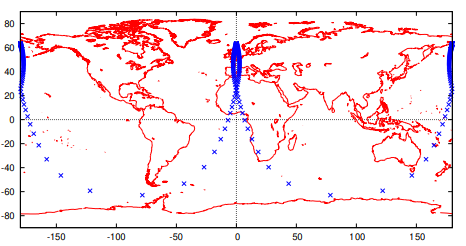
\includegraphics[width=0.8\textwidth]{portada.PNG}\par}
    \vspace{1cm}
    %{\scshape\Huge Universitat Autònoma de Barcelona\newline Facultat de Ciències \par}
    \vspace{1cm}
    {\Large \itshape Gerard Lahuerta Martín \par}
    \vspace{1cm}
    {\Large 4 de Juny del 2021\par}
\end{titlepage}

\justifying

\newpage
\setcounter{page}{2}
\pagestyle{plain}
\tableofcontents
\cleardoublepage
\addcontentsline{}{chapter}{}


\section{Introducció}
\subsection{Motivació del treball}
Aquest treball ha estat motivat pel \textbf{Departament de Control de Missió de l'Agència Espacial Catalana ($\mathbf{AEC}$)} en requerir una eina de software que li permeti determinar la posició d'un satèl·lit artificial en el seu
pla orbital.
\subsection{Metodologia}
\subsubsection{Explicació de la metodologia}
La metodologia aplicada a l'hora de programar la biblioteca que sol·licitava l'\textbf{$\mathbf{AEC}$} ha estat la següent:
\begin{enumerate}
\item Llenguatge de programació ràpid i eficient
\newline
Utilitzem el llenguatge C gràcies a la rapidesa en els càlculs i l'alta eficiència.
\item Fàcil d'executar
\newline
La programació ha estat orientada a la fàcil utilització d'aquest per tal de ser intuïtiva, a més, s'afegeix el manual d'ús del software per les consultes necessàries.
\item Fàcil modificació
\newline
El programa està forçament comentat i enfocat per a ser fàcilment intuïtiu per si calgués alguna modificació a posterior i, així, facilitar la tasca.
\item Màxima optimització possible a la vegada que eficàcia i fiabilitat dels càlculs
\newline
Combinem la velocitat del mètode de Newton amb la robustesa del mètode de bisecció en els càlculs orbitals.
\end{enumerate}
\newpage
\subsubsection{Comentaris}
El disseny de les rutines ha estat pensat i implementat per a evitar els càlculs i interaccions innecessàries. També, s'ha evitat la creació de rutines i variables redundants per a obtenir la millor optimització possible.
\newline
Tal com hem comentat anteriorment, per tal d'evitar confusions i ajudar a l'enteniment de les accions del programa s'han implementat línies de codi comentat, aquestes expliquen els conceptes més ambigus del programa i estan localitzades al costat de cada línia on s'ha cregut necessària una explicació.
\newline
També, afegir que els càlculs utilitzats en la utilitat $kpl2nu.c$ (explicats a \textcolor{navy}{Secció 1.3}) han estat els proporcionats per l'\textbf{$\mathbf{AEC}$} i han estat aplicats tal com ens els han proporcionat i demanat que s'apliquin.

\subsubsection{Informació d'interès}
La biblioteca ha estat programada amb l'editor d'ús públic Notepad++, encara que pot ser modificat en altres editors com podrien ser l'editor de notes o d'altres més complexos com VisualStudio.
\newline
Durant la programació de les rutines s'ha ideat un programa per testejar el correcte funcionament de la biblioteca i així en cas de possibles errors poder comprovar el correcte funcionament d'aquesta.
\newline
L'ús d'aquest test que està anomenat com $bisnwt\_test.c$
és fàcilment executable i és explicat més a fons a la \textcolor{navy}{Secció 2.3}.
\newpage
\subsection{Càluls utilitzats en la utilitat $kpl2nu.c$}
Per a fer els càlculs orbitals se'ns és necessari les següents dades:
\begin{wrapfigure}{l}{0.5\textwidth}
\begin{center}
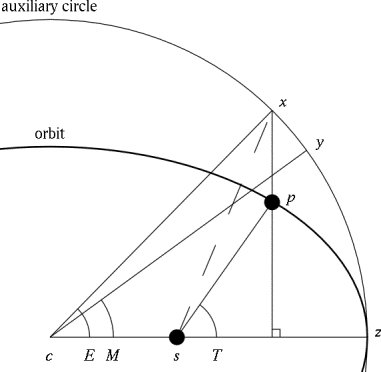
\includegraphics[width=0.5\textwidth]{Kepler's-equation-scheme.png}
\end{center}
\caption{Relació entre anomalies}
\label{fig:relacio-anomalies}
\end{wrapfigure}
\begin{itemize}
\item [$\bullet$] \textbf{Anomalia Mitjana: $M$}
\newline
% Sabem que $M$ és:
$$M=2\pi\frac{t-t_p}{T}$$
\item [$\bullet$] \textbf{Anomalia Excentrica: $E$}
\newline
%Càlculem $E$ amb la formula de Kepler:
$$M=E-e\sin{E}$$
\item [$\bullet$] \textbf{Anomalia Vertadera: $\nu$}
\newline
%Obtenim $\nu$ a partir de:
$$\nu=\arccos{\frac{e-\cos{E}}{e\cos{E}-1}}$$
\end{itemize}
\textcolor{white}{hola}
\\
\\
On $t, tp, T$ i $e$ són respectivament el temps actual, el temps que tarda en passar pel perigeu (un dels màxims de l'òrbita el·líptica), el període de l'òrbita i l'excentricitat de l'el·lipse.
\newline
Recalcar que: $t\in[0,+\infty)$, $tp\in\Re$, $T\in\Re$ i $e\in[0,1)$ són coneguts i proporcionats per l'$\mathbf{EAC}$.
També afegir que: $M\in\Re$, $E\in[0,2k\pi]$ i $\nu\in[0,2k\pi]$, essent $k\in\mathbb{N}$
\newpage
\section{Explicació de la biblioteca $bisnwt.c$}
En aquest capítol parlarem a fons sobre l'estructura, els materials que implementa, el funcionament, les estratègies utilitzades i el correcte ús i execució del programa.
\subsection{Implementació}
La biblioteca està pensada per a ser implementada en els entorns d'execució de l'$\mathbf{EAC}$.
\newline
L'únic mètode que s'inclou a la biblioteca (del qual parlem a continuació) pot ser utilitzat independentment del programa que l'implementi i no precisa cap altra eina externa més enllà de la llibreria \textit{math.h} del conjunt de llibreries del llenguatge C.
\subsection{Funcionament}
El funcionament del mètode $bisnwt$ és senzill. Aplica inicialment el mètode de bisecció per a trobar un interval menor a un valor $\delta$ introduït per a desprès aplicar amb el mètode de Newton per a trobar l'arrel (així ens assegurem una millor viabilitat i eficiencia en els càlculs). \newline
Finalment, si el mètode de newton després de \textit{maxit} iterats (introduït també com a paràmetre) no ha convergit, el redueix el valor de $\delta$ en la mitad i es repeteix el procés fins que el mètode Newton convergeixi o l'interval sigui menor que un tolerancia (\textit{tol}) prèviament també introduïda.\newline\newline
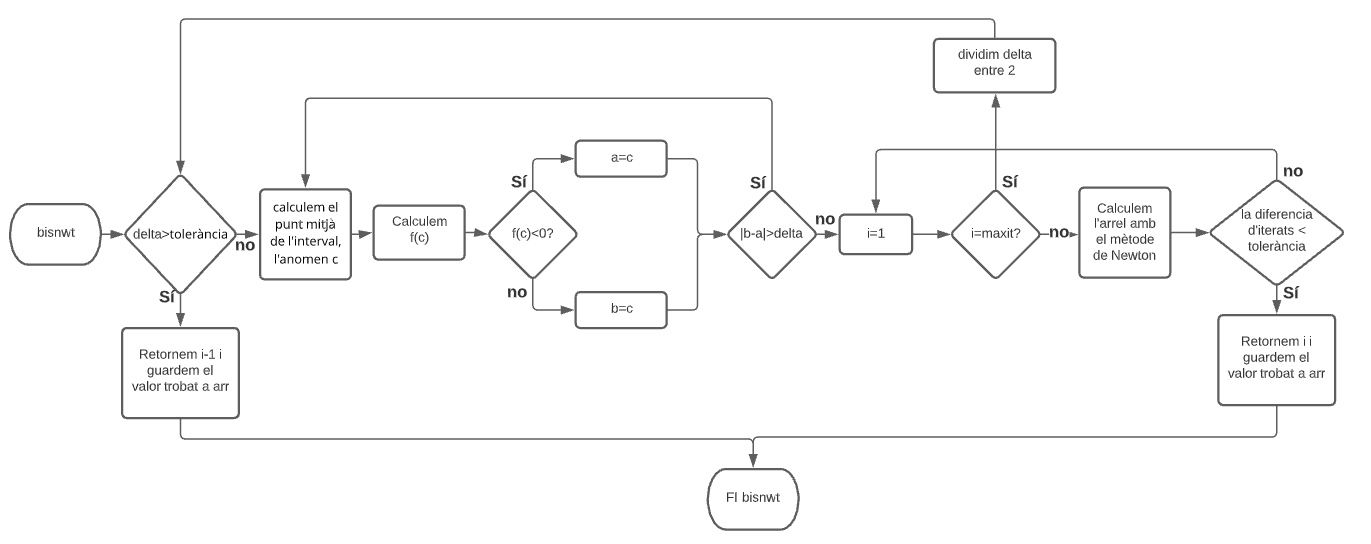
\includegraphics[width=1\textwidth]{diagrama-bisnwt.PNG}
\newpage
\subsection{Testatge de la biblioteca: $test$ i $bisnwt\_test.c$}
Expliquem a continuació el programa $bisnwt\_test.c$ i la correcta implementació de la biblioteca en els codis de programació de l'$\mathbf{EAC}$ així com en el mateix codi.
\subsection{Compilació de la utilitat de testatge: $bisnwt\_test.c$}
Per a implementar a biblioteca $bisnwt.h$ en qualsevol codi en C cal a l'inici del codi escriure la comanda següent:
\begin{verbatim}
#include "bisnwt.h"
\end{verbatim}
Una vegada escrita la comanda el programa implementarà l'extensió al codi.
\newline
Per a compilar $test\_bisnwt.c$ i obtenir la utilitat $test$ es pot utilitzar l'arxiu \textit{MakeFile} que s'inclou. \newline
Aquest es pot utilitzar de les maneres següents:
\begin{itemize}
\item [$\circ$] \textbf{Si es tracta del sistema Operatiu Unix}, en la consola/terminal de l'ordinador executar la comanda \textit{make -f Makefile.txt} per crear l'executable $test$.
\newline
Anàlogament, executar la comanda \textit{clean -f Makefile.txt} per netejar \textit{d'arxius objecte} innecessaris el directori de treball o \textit{realclean -f Makefile.txt} per esborrar tot el treball fet per l'arxiu Makefile.
\item [$\circ$] \textbf{Si es tracta del sistema Operatiu Windows}, en la consola/terminal de \textit{mingw-w64} executar la comanda \textit{mingw32-make -f Makefile$\_$Windows.txt} per crear l'executable \textit{test.exe}.
\newline
Anàlogament, executar la comanda \textit{minw32-make clean -f Makefile$\_$Windows.txt} per netejar d'arxius objecte innecessaris el directori de treball o \textit{minw32-make realclean -f Makefile$\_$Unix.txt} per esborrar tot el treball fet per l'arxiu Makefile.
\end{itemize}
Si no s'utilitza l'arxiu Makefile, es pot compilar els arxius que continguin aquesta biblioteca amb la comanda següent al terminal/consola:
\begin{verbatim}
gcc -o nom_del_executable -Wall nom_del_programa.c bisnwt.c -lm
\end{verbatim}
\newpage
Per obtenir l'executable que ens interesa en aquest cas utilitzem la comanda abans explicada,
\begin{verbatim}
gcc -o test -Wall test_bisnwt.c bisnw.c
\end{verbatim}
O també podem utilitzar l'arxiu Makefile amb:
\begin{verbatim}
make -f test Makefile.txt
\end{verbatim}
Analogament en cas de Windows, aplicar la comanda explicada pel sistema operatiu amb l'afegit de la comanda \textit{test} abans del nom de l'arxiu.
\subsection{Output i executable $test$}
Per tal d'assegurar el funcionament correcte de la biblioteca hem posat a disposició de l'$\mathbf{EAC}$ el codi $test\_bisnwt$ que té com a objectiu assegurar que el mètode que actualment conté la biblioteca funcioni de manera correcta.
\newline
El programa $test\_bisnwt.c$ és molt senzill, únicament crida la funció que conté $bisnwt.h$ per fer uns càlculs de prova i eventualment mostrar-los per pantalla.
\newline
Per a executar la utilitat cal introduir pel terminal les següents comandes i comparar-les amb els respectius outputs:
\begin{itemize}
\item \textbf{test \hspace{0.5em} -9 \hspace{0.5em} 1 \hspace{0.5em} 10 \hspace{0.8em} 1e-12 \hspace{0.5em} 10}
\begin{verbatim}
valor: 0.6931471805599453 estat del valor: 7
\end{verbatim}
\item \textbf{test \hspace{0.5em} -9 \hspace{0.5em} 1 \hspace{0.5em} 2.5 \hspace{0.5em} 1e-12 \hspace{0.5em} 10}
\begin{verbatim}
valor: 0.6931471805599453 estat del valor: 7
\end{verbatim}
\item \textbf{test \hspace{0.5em} -9 \hspace{0.5em} 1 \hspace{0.5em} 0.1 \hspace{0.5em} 1e-12 \hspace{0.5em} 10}
\begin{verbatim}
valor: 0.6931471805599453 estat del valor: 5
\end{verbatim}
\end{itemize}
\newpage
\section{Explicació de la utilitat}
\subsection{Funcionament de $kpl2nu.c$}
En aquesta secció explicarem el funcionament del programa $kpl2nu.c$, el seu funcionament intern i les seves dependències.
\subsection{Dependències}
Primerament cal esmentar i explicar les necessitats i dependències del programa $kpl2nu.c$.
\newline
Aquest requereix la biblioteca solicitada i explicada anteriorment ($bisnwt.h$). Per altra banda, per a dur a terme els càlculs se l'introdueix com arguments en l'execució els valors de $e$, $T$, $M0$, $tf$ i $nt$ on:
\begin{itemize}
\item [$\blacktriangleright$] \textbf{Variable \textit{e}:} double que guardarà l'excentricitat de l'el·lipse que traça el satel·lit.
\item [$\blacktriangleright$] \textbf{Variable \textit{T}:} double que guardarà el valor del període de l'òrbita del satel·lit.
\item [$\blacktriangleright$] \textbf{Variable \textit{M0}:} double que guardarà el valor de l'anomalia mitjana inicial (en $t_0=0$).
\item [$\blacktriangleright$] \textbf{Variable \textit{tf}:} double que guardarà el temps final en la trajectora del programa.
\item [$\blacktriangleright$] \textbf{Variable \textit{nt}:} integuer que guardarà el nombre d'intervals a càlcular de l'òrbita.
\end{itemize}
Amb totes aquestes dades, el programa ya pot treballar en calcular la traça de la trayectoria del satèl·lit.
\newpage
\subsubsection{Explicació de $kpltnu2.c$}
El funcionament del programa, en concepte és senzill. A partir de les dades inicials calcula el nombre d'intervals en els quals calcular on es troba el satel·lit en la seva òrbita per així, una vegada calculats tots els intervals, mostrar les dades per pantalla.
\newline
Per poder calcular l'anomalia Excèntrica $E$ utilitzem la biblioteca $bisnwt.h$ cridant el mètode \textit{bisnwt}.
\begin{wrapfigure}{l}{1\textwidth}
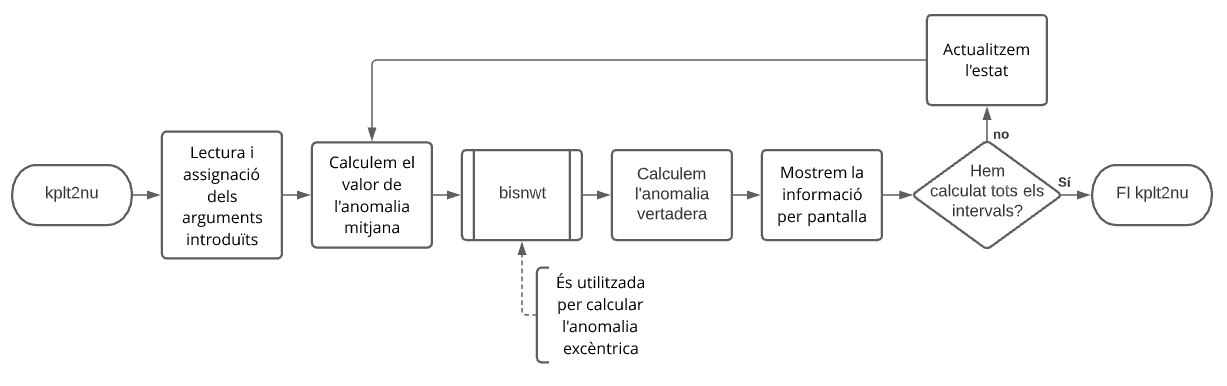
\includegraphics[width=1\textwidth]{Diagrama-kplt2nu.PNG}
\caption{Diagrama del codi kplt2nu}
\label{fig:my_label}
\end{wrapfigure}
\textcolor{white}{hola}\newline\newline\newline\newline\newline\newline\newline\newline\newline\newline
Cal recalcar que els valors que fan referència al màxim d'iteracions $maxit$, la $\delta$ així com la tolerancia $tol$ són ja paràmetres definits en el codi; concretament $100$, $0.01$ i $10^{-12}$ respectivament.
\newline
També afegir que a l'hora de programar $kpl2nu.c$ es va programar per necessitat del càlculs dues funcions ($Kepler\_fxE$ i $Kepler\_dfxE$) que són les introduïdes com apuntadors a funcions en el mètode $bisnwt$ que, per a poder obtenir totes les dades necessàries, se'l passà un l'adreça de memoria de l'estructura $dades\_kpl$ que conté l'excentricitat de l'el·lipse $e$ i l'anomalia mitjana actualizada per la posició que es vol calcular $M$.
\newpage
\section{Execució $kplt2nu$}
\subsubsection{Compilació de $kpl2nu.c$}
Per a compilar $kpl2nu.c$ i obtenir l'executable $kplt2nu$ es pot utilitzar la comanda següent:
\begin{verbatim}
gcc -o kplt2nu.c -Wall kplt2nu.c bisnw.c
\end{verbatim}
O també podem utilitzar l'archiu Makefile amb:
\begin{verbatim}
make -f kplt2nu Makefile.txt
\end{verbatim}
Anàlogament en cas de Windows, aplicar la comanda explicada pel sistema operatiu amb l'afegit de la comanda
\subsubsection{Output del programa}
L'output de la utilitat són tres columnes de dades que són impreses per pantalla ordenada de la següent manera:
$$
\begin{array}{ccc}
t_0 & M_0 & \nu_0 \\
t_1 & M_1 & \nu_1 \\
\vdots & \vdots & \vdots \\
t_{nt} & M_{nt} & \nu_{nt}
\end{array}$$
Essent $t$ el temps, $M$ l'anomalia mitjana, $\nu$ l'anomalia excèntrica i $nt$ el valor d'intervals en el que dividir l'òrbita del satèl·lit.
\newline
Pel fet que l'output mostrat tendeix a ser molt gran, es recomana afegir en el moment de l'execució una redirecció d'entrada a un fitxer que guardi tota la informació.
\newpage
\section{Anàlisis de les dades obtingudes}
Per analitzar millor les dades obtingudes s'hi ha optat en utilitzar el programa informàtic $gnuplot$. \newline
Per a poder representar l'òrbita sobre el mapa terrestre del satèl·lit cal executar les següents comandes dins del terminal de $gnuplot$.
\begin{verbatim}
> load 'ctants.gnu'
> lonesp=0 # longitud del lloc que espia
> xc=0.74105 # excentricitat
> T=dias/2 # període de l'òrbita (mig dia sideri)
> i=63.4*(pi/180) # inclinació de l'òrbita (en radians)
> tf=dias # simulem durant un dia
> nt=333 # a la traça es representen 333 punts
> load 'dibgte.gnu'
\end{verbatim}
En cas que es vulgui representar un diagrama amb l'altura que adquireix el satèl·lit cal executar després de les comandes anteriors la línia següent:
\begin{verbatim}
> set autoscale ; plot 'gtrk.txt' u 1:(r($3)) w lp
\end{verbatim}
Amb aquest exemple d'aquí s'obté les següents imatges:
\begin{figure}
\centering
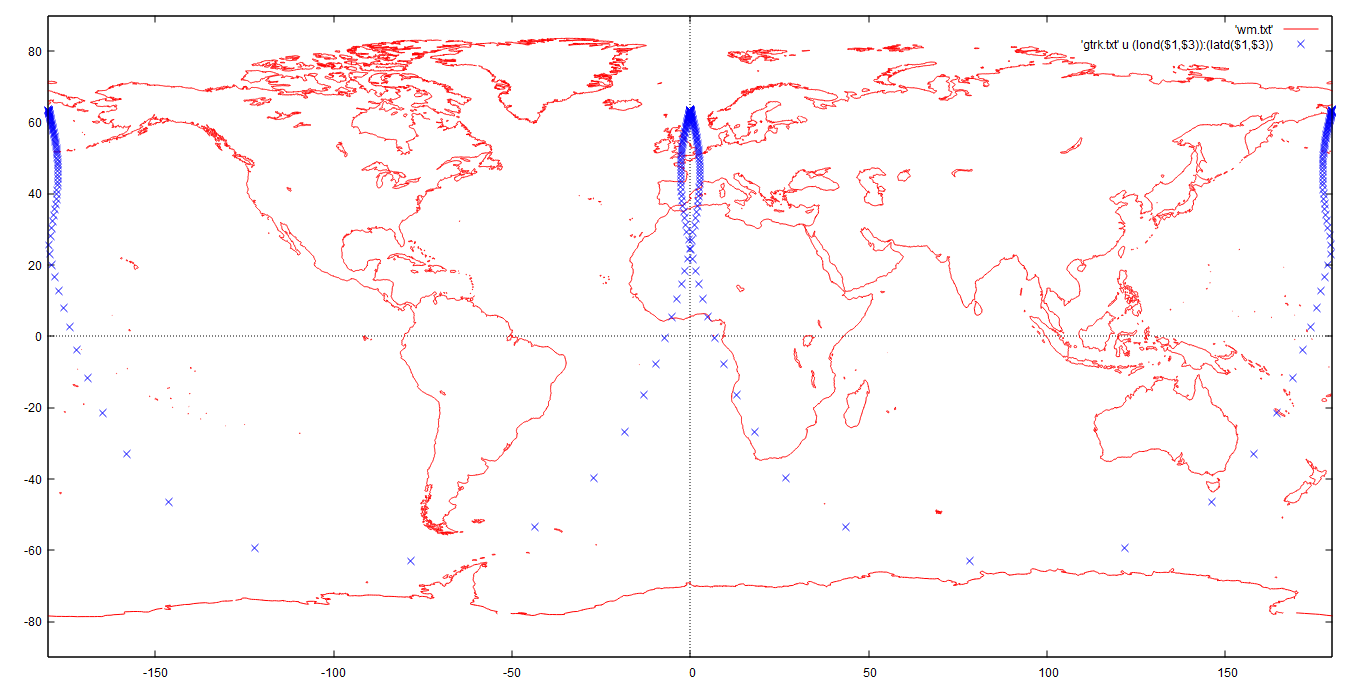
\includegraphics[width=1\textwidth]{orbita_principal.png}
\caption{Traça de la configuració d'exemple}
\label{fig:traç-exemp}
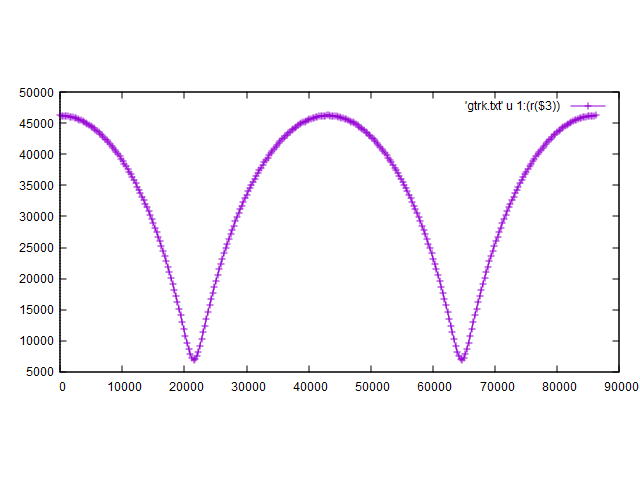
\includegraphics[width=1\textwidth]{altitud_principal.png}
\caption{Gràfic de l'altura de la configuració d'exemple}
\label{fig:alti-exemp}
\end{figure}
\newpage
\textcolor{white}{hola}
\newpage
\begin{titlepage}
\centering
{
\includegraphics[width=1\textwidth]{topsecret.PNG}\par}
\vspace{5cm}
{\Huge Propostes sobre d'investigació i espionatge per l'$\mathbf{EAC}$\par}
\end{titlepage}
Com a part de la nostra tasca en la programació de la utilitat $kplt2nu$, hem fet una recopilació de països als que l'$\mathbf{EAC}$ podria estar interesada en investigar/espiar les seves activitats aprofitant les qualitats de les òrbites Molniya.
\newline
Una de les possibilitats de llocs a estudiar serien Nord Corea i els Estats Units d'Amèrica, que poden ser espiats mitjançant una òrbita amb una excentricitat $e=0.5$, tingui un període de $T=\frac{\text{dia sireri}}{3}$ i una longitud del meridià $lonesp=-4$. Tot així no recomenem del tot aquesta configuració orbital a causa del gran risc de caure en l'atmosfera a causa del fregament amb ella (ja que hi passa molt prop d'ella).\\
Per altra banda, també es proposa l'espionatge al Regne Unit mitjançant un satèl·lit que orbiti amb una excentricitat $e=0.543210987654$ una longitud de meridia $lonesp=0$ i un període d'òrbita $T=\text{dia sireri}$. Aquesta órbita s'allunya suficientment de l'atmosfera i pot espiar el Regne Unit a la vegada que envia la informació que es rep a la seu de control de l'$\mathbf{EAC}$.\\
Finalment, l'òrbita més factible és la que té una excentricitat de $e=0.498765678923$, un període $T=\frac{\text{dia sireri}}{2}$ i una longitud del meridia $lonesp=0$. Aquesta està feta per a observar els moviments en l'estret de Bering entre Rusia i Estats Units.
\newpage
\begin{figure}
\centering
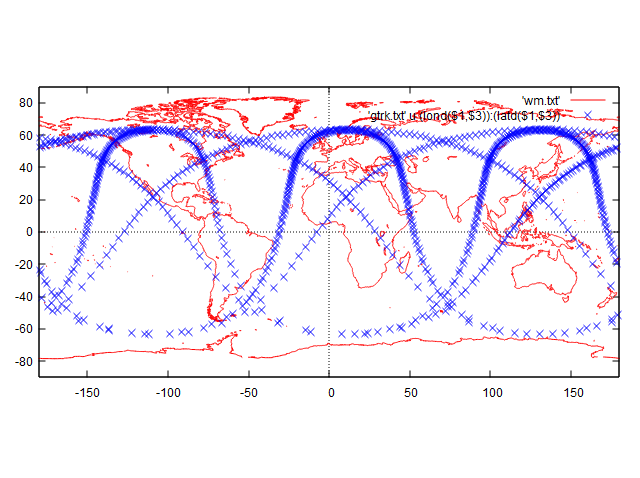
\includegraphics[width=0.8\textwidth]{orbita-USA-KPOP-EU.png}
\caption{Traça de l'òrbita per a espiar a Nord Corea i USA amb 1000 punts}
\label{fig:my_label}

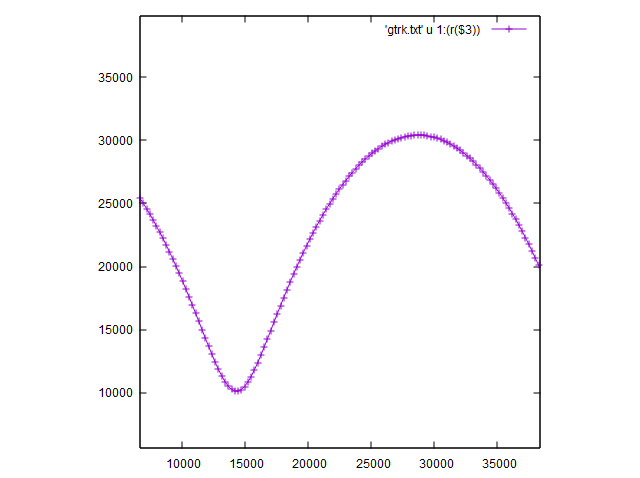
\includegraphics[width=0.7\textwidth]{altitud-USA-KPOP_EU.png}
\caption{Altituds de l'òrbita per a espiar a Nord Corea i USA amb 1000 punts}
\label{fig:relacio-anomalies}
\end{figure}
\begin{figure}
\centering
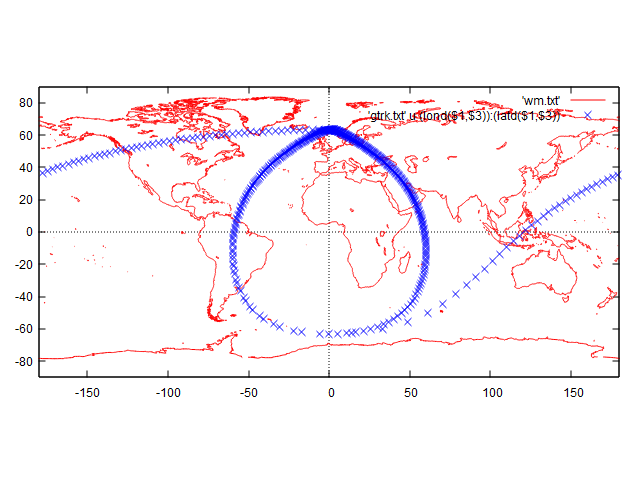
\includegraphics[width=0.8\textwidth]{orbita-UK.png}
\caption{Traça de l'òrbita per a espiar el Regne Unit amb 1000 punts}
\label{fig:my_label}

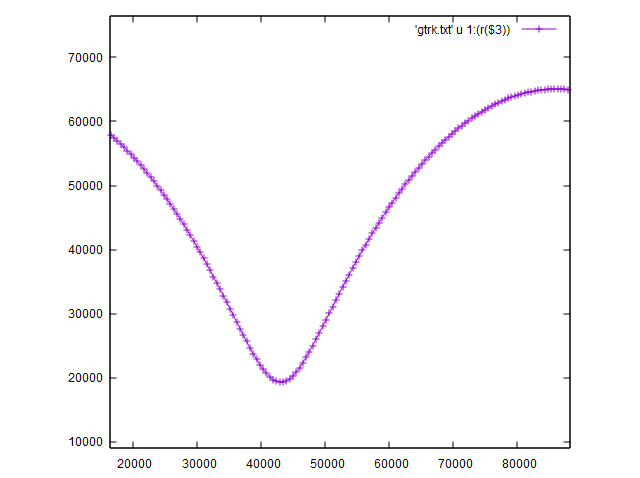
\includegraphics[width=0.7\textwidth]{altitud-UK.png}
\caption{Altituds de l'òrbita per a espiar el Regne Unit amb 1000 punts}
\label{fig:relacio-anomalies}
\end{figure}
\begin{figure}
\centering
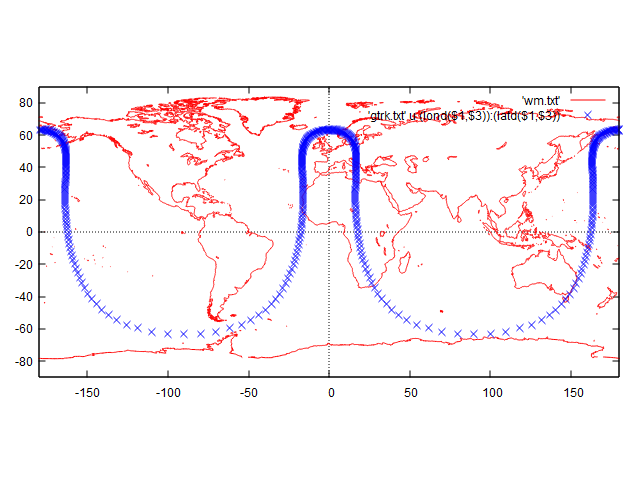
\includegraphics[width=0.8\textwidth]{orbita-beijing.png}
\caption{Traça de l'òrbita per a espiar l'estret de Bering amb 1000 punts}
\label{fig:my_label}

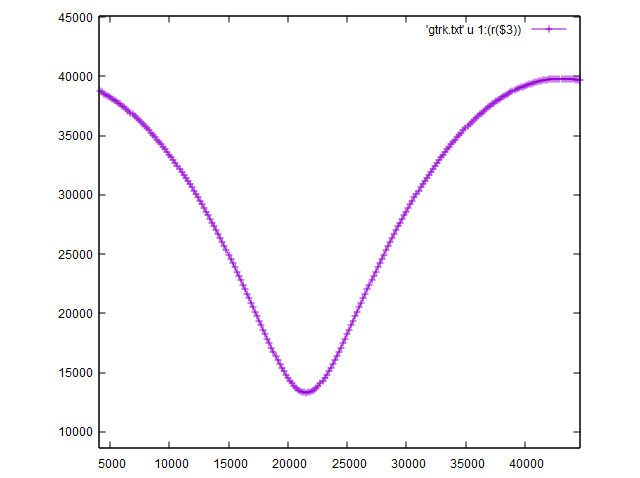
\includegraphics[width=0.7\textwidth]{altitud-beijing.png}
\caption{Altitud de l'òrbita per a espiar l'estret de Bering 1000 punts}
\label{fig:relacio-anomalies}
\end{figure}
\end{document}